% Modern editorial, markup and figure/layout contributions: CC-BY-SA-4.0.
% Historical text and illustrations: Leonhard Euler (1744), public domain.
% Component scope and upstream attribution: see RIGHTS.md.
% Manual vector redrawing after E65, Tabula IV. Schematic coordinates; original point relations retained.
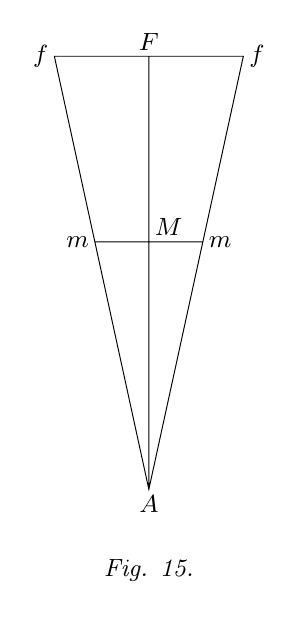
\begin{tikzpicture}[x=1cm,y=1cm,line width=.35pt,font=\small]
\draw (0,0)--(-1.2,5.5)--(1.2,5.5)--cycle (0,0)--(0,5.5) (-.6857,3.1429)--(.6857,3.1429);
\node[below,inner sep=2pt] at (0,0) {$A$};
\node[above,inner sep=2pt] at (0,5.5) {$F$};
\node[left,inner sep=2pt] at (-1.2,5.5) {$f$};
\node[right,inner sep=2pt] at (1.2,5.5) {$f$};
\node[above right,inner sep=2pt] at (0,3.1429) {$M$};
\node[left,inner sep=2pt] at (-0.6857,3.1429) {$m$};
\node[right,inner sep=2pt] at (0.6857,3.1429) {$m$};
\node[anchor=north] at ([yshift=-4mm]current bounding box.south) {\textit{Fig. 15.}};
\end{tikzpicture}
